% arara: pdflatex: { synctex: yes }
% arara: makeindex: { style: ctuthesis }
% arara: bibtex

% The class takes all the key=value arguments that \ctusetup does,
% and a couple more: draft and oneside
\documentclass[twoside]{ctuthesis}

\ctusetup{
%	preprint = \ctuverlog,
%	mainlanguage = english,
	titlelanguage = czech,
	mainlanguage = czech,
	otherlanguages = {slovak,english},
	title-czech = {Identifikace 6-osého průmyslového robotu},
	title-english = {Identification of a 6-axis industrial robot},
%	subtitle-czech = {Cesta do tajů kdovíčeho},
%	subtitle-english = {Journey to the who-knows-what wondeland},
	doctype = M,
	faculty = F3,
	department-czech = {Katedra řídicí techniky},
	department-english = {Department of control engineering},
	author = {Bc. Andrej Suslov},
	supervisor = {Ing. Martin Ron},
%	supervisor-address = {Ústav X, \\ Uliční 5, \\ Praha 99},
%	supervisor-specialist = {John Doe},
%	fieldofstudy-english = {Mathematical Engineering},
%	subfieldofstudy-english = {Mathematical Modelling},
	fieldofstudy-czech = {Systémy a řízení},
    subfieldofstudy-czech = {Kybernetika a robotika},
	keywords-czech = {robot, model, identifikace, parametr, průmysl, energie, spotřeba, databáze},
    keywords-english = {robot, model, identification, parameter, industry, energy, consumption, database},
	day = 24,
	month = 5,
	year = 2017,
	specification-file = {Suslov-Andrej_zadani.pdf},
	front-specification = true,
	front-list-of-figures = true,
	front-list-of-tables = true,
%	monochrome = true,
%	layout-short = true,
}

\ctuprocess

\addto\ctucaptionsczech{%
	\def\supervisorname{Vedoucí práce}%
	%\def\subfieldofstudyname{Studijní program}%
}

\ctutemplateset{maketitle twocolumn default}{
	\begin{twocolumnfrontmatterpage}
		\ctutemplate{twocolumn.thanks}
		\ctutemplate{twocolumn.declaration}
		\ctutemplate{twocolumn.abstract.in.titlelanguage}
		\ctutemplate{twocolumn.abstract.in.secondlanguage}
		\ctutemplate{twocolumn.tableofcontents}
		\ctutemplate{twocolumn.listoffigures}
	\end{twocolumnfrontmatterpage}
}

% Theorem declarations, this is the reasonable default, anybody can do what they wish.
% If you prefer theorems in italics rather than slanted, use \theoremstyle{plainit}
\theoremstyle{plain}
\newtheorem{theorem}{Theorem}[chapter]
\newtheorem{corollary}[theorem]{Corollary}
\newtheorem{lemma}[theorem]{Lemma}
\newtheorem{proposition}[theorem]{Proposition}

\theoremstyle{definition}
\newtheorem{definition}[theorem]{Definition}
\newtheorem{example}[theorem]{Example}
\newtheorem{conjecture}[theorem]{Conjecture}

\theoremstyle{note}
\newtheorem*{remark*}{Remark}
\newtheorem{remark}[theorem]{Remark}

%\setlength{\parskip}{5ex plus 0.2ex minus 0.2ex}
\setlength{\parskip}{2ex plus 0.2ex minus 0.2ex}

% Abstract in Czech
\begin{abstract-czech}
Tato práce se zabývá odvozením a identifikací modelu 6-osého průmyslového robotu. Tento model je následně použit k predikci jeho energetické spotřeby. V první části 
je představen robotický systém, který je předmětem modelování. Poté je popsán způsob měření elektrického výkonu a popsána vytvořená aplikace pro přípravu dat dlouhodobého měření spotřeby elektrické energie. V další části jsou nastíněny způsoby odvození dynamických rovnic robota. Nasleduje kapitola zabývající se různými způsoby identifikace a jejich vzájemným srovnáním. V následující části je popis vytvoření a identifikace modelu robota a jeho porovnání s reálnými změřenými hodnotami. Dále se práce zabývá způsobem měření elektrického výkonu robota a konečným porovnáním modelem predikovaných hodnot s reálným měřením. V poslední části se práce zabývá analýzou vlivu odchylek identifikovaných parametrů na přesnost modelu.    
\end{abstract-czech}

% Abstract in English
\begin{abstract-english}
This thesis is focused on derivation and identification of a model of a 6-axis industrial robot. Derived model is then used for prediction of robot's energy consumption. In the first part there is an introduction of a robotic system to be modelled. Then the way of measurement of electrical power and an application for preparation of data of long-term measurement of energy consumption is described.
In the next part there are outlined some approaches to derive dynamic equations of a robot. It is followed by different ways of parameter identification and their comparison. Next part is focused on actual creation and identification of robot's model and its comparison with measurements. Further, the thesis is focused on measurement of robot's electrical power and final comparison between preduction and real measuremet. Finally, there is a description of analysis of influence of deviations in identified parameters on model precision. 

\end{abstract-english}

% Acknowledgements / Podekovani
\begin{thanks}
Rád bych tímto poděkoval svému vedoucímu práce panu Ing. Martinu Ronovi za jeho cenné rady a vedení při tvorbě této práce. Jeho pomoc byla velikým přínosem během celého průběhu jejího vzniku. 

Dále bych rád poděkoval svým nejbližším, rodině a přítelkyni, za jejich podporu během tvorby této práce, během celého studia i osobního života. 

\end{thanks}

% Declaration / Prohlaseni
\begin{declaration}
Prohlašuji, že jsem předloženou práci vypracoval samostatně, a že jsem uvedl veškeré informační zbroje v souladu s Metodickým pokynem o dodržování etických principů při přípravě vysokoškolských závěrečných prací.
\\
\\
\\
V Praze, dne \ctufield{day}.~\monthinlanguage{title}~\ctufield{year}\\
\\
\\\hbox{}
\dotfill\hfill
\end{declaration}

% Only for testing purposes
\listfiles
\usepackage[pagewise]{lineno}
\usepackage{lipsum,blindtext}
\usepackage[square,numbers]{natbib}
\usepackage{mathrsfs} % provides \mathscr used in the ridiculous examples
%\usepackage[showframe]{geometry}
\usepackage{amsmath}
\usepackage{graphicx}
%\usepackage{subfig}
\usepackage{newunicodechar}
\usepackage{siunitx}
\usepackage{wrapfig}
\usepackage[utf8]{inputenc}
\usepackage{amsmath,bm}
\usepackage{courier}
\usepackage{caption}
\usepackage{subcaption}
\usepackage{float}
\usepackage{changepage}   

\graphicspath{{./img/}}

\begin{document}

\maketitle

\newcommand{\vect}[1]{\boldsymbol{#1}}


%!TEX ROOT=ctutest.tex

\chapter{Úvod}


%Cílem této práce je vytvoření matematického modelu průmyslového robotického manipulátoru za účelem modelování jeho spotřeby elektrické energie při výkonu daných robotických operací. Tato data by poté měla sloužit pro další identifikaci.

%Modelování průmyslových robotů již bylo předmětem mnoha prací a projektů a to už od jejich návrhu a prvních použití. Nejčastěji tyto modely slouží pro návrh řízení robota nebo jeho optimalizaci. Tato práce je zaměřena na modelování robota a identifikaci z hlediska jeho spotřeby elektrické energie. Protože dynamické parametry robota často nejsou známy, je nejprve nutné tyto parametry identifikovat.

%Identifikací dynamických parametrů se již zabývalo několik prací. V článcích \cite{par_iden_rob}\cite{clos_dyn_par} je použita identifikace dynamických parametrů metodou nejmenších čtverců. Práce \cite{dyn_mod_ind}\cite{dyn_ind_mits} se zabývají identifikací touto metodou robota Mitsubishi PA-10. Jiným způsobem se postupuje v článcích \cite{dyn_ind_man} a \cite{akeel}, které se zabývají identifikací systému pomocí 3D modelu. V této práci je k identifikaci je použita metoda identifikace pomocí nejmenších čtverců.

%Průmyslové robotické manipulátory jsou dnes již nedílnou součástí průmyslové sféry. Na rozdíl od jednoduchých jednoúčelových průmyslových strojů, které jsou úzce specializované jen na jeden typ operace, jsou průmyslové roboty víceúčelové a jsou schopny vykovávat téměř libovolnou operaci. Jsou omezeny jen vlastní geometrií, uspořádáním pracovního prostoru ve které se provozují a mechanickými vlastnostmi aktuátorů a jednotlivých prvků robota. Díky těmto vlastnostem je jeden průmyslový robot schopen vykovávat operace, ke kterým by jinak bylo potřeba více strojů, a to jen změnou programu.

%Dnes se roboty v průmyslu používají pro mnoho typů operací. Patří mezi ně svařování, montáž, manipulace s materiálem, lakování, vrtání a mnoho dalších.









%!TEX ROOT=ctutest.tex

\chapter{Robotický systém}



Měření průběhů dynamických parametrů se provádí na průmyslovém robotu KUKA KR5 Arc \cite{kuka_url} od společnosti KUKA Roboter GmbH (obr. \ref{kuka_kr5_pic}). Jedná se o 6-ti osového robota, který má 6 rotačních os poháněných servomotory. Osy robota jsou uspořádány tak, že jsou schopny napodobit stavbu a pohyb lidské paže. Konfigurace os robota je zobrazena na obrázku \ref{kuka_kr5_axes_pic}. 

\begin{figure}[ht]
\includegraphics[width=0.45\textwidth]{PR_KR5_arc_02}
\caption{Robot KUKA KR5 Arc. Převzato z \cite{kuka_datasheet_url}.}
\label{kuka_kr5_pic}
\end{figure}

Tento robot s hmotností 127 kg a základní nosností 5 kg patří mezi lehčí průmyslové roboty. Byl vyvinut primárně pro aplikace vyžadující vysokou přesnost polohování, jako je obloukové svařování a přesná manipulace s lehkými pevnými předměty. Je určen pro montáž na zem ve vnitřních prostorách.

\begin{figure}[ht]
\includegraphics[width=0.65\textwidth]{kuka_kr5_axes}
\caption{Konfigurace os robota. Převzato z \cite{kuka_datasheet_url}.}
\label{kuka_kr5_axes_pic}
\end{figure}

Jako pohony os jsou použity synchronní servopohony s permanentními magnety (PMSM). Pro zvýšení točivého momentu motorů a přesnosti polohování jsou motory opatřeny převodovkou. Podrobnější informace je možné nalézt v katalogovém listu \cite{kuka_datasheet_url}.
\chapter{Měření elektrického výkonu}

Správnost odvozeného a identifikovaného modelu robota je potřeba ověřit a porovnat se skutečným měřením elektrického výkonu. Měření výkonu bylo provedeno podle schématu na obrázku \ref{mereni_vykonu_pic}. Měřicí sestava je připojena na svorky napájecího vedení mezi elektrickou zásuvkou a skříní s řídicím systémem a napájením robota. Sestava je tvořena měřicí kartou WAGO-I/O-SYSTEM 750 připojenou k průmyslovému PLC Siemens S7-300 CPU 315-2PN/DP. Měřicí karta WAGO obsahuje svorky pro měření napětí a proudu v třífázové síti. 

\begin{figure}[ht]
\includegraphics[width=0.9\textwidth]{mereni_vykonu_obr}
\caption{Schéma zapojení soustavy pro měření výkonu.}
\label{mereni_vykonu_pic}
\end{figure}

Pro účely měření výkonu robotu KUKA KR5 Arc byla karta nakonfigurována pro měření činného výkonu na každé jednotlivé fázi zvlášť. Výsledný celkový výkon je poté podle vzorce \ref{3ph_power_eq} roven součtu výkonů všech jednotlivých fází. Měření výkonu je prováděno s přesností na desetiny wattu. Vzorkovací perioda měření je 40 ms. 

\section{Měřicí karta WAGO-I/O-SYSTEM 750}

Měřicí karta WAGO-I/O-SYSTEM 750 [\cite{wago}] je určena pro měření elektrických veličin v třífázové síti. Je navržena pro použití v průmyslovém prostředí v kombinaci s průmyslovým počítačem PLC. 

Karta je opatřena svorkami pro měření napětí a proudu na každé fázi zvlášť. Měření proudu je prováděno pomocí proudového transformátoru převádějícího měřený proud na napětí. 

Kartu je možné nakonfigurovat pro současné měření až čtyř elektrických veličin jako je stejnosměrné (DC) a střídané (AC) napětí, proud, výkon, frekvence, fázový posuv a další, a to pro každou fázi zvlášť. Navíc je karta schopna provádět analýzu harmonických složek signálu pro vybranou fázi a to až pro 3 vybrané harmonické složky z rozsahu 1. a 41. harmonické. 

\begin{figure}[ht]
    \includegraphics[width=0.3\textwidth]{wago_obr}
    \caption{Měřicí karta WAGO-I/O-SYSTEM 750.}
    \label{wago_pic}
\end{figure}

Změřené veličiny posílá karta přímo na vstupy připojeného PLC, které je dále zpracovává. Měřicí karta se vstupními svorkami je na obrázku \ref{wago_pic}. Technické parametry a podrobnější informace o použití karty je možné nalézt v jejím manuálu [\cite{wago}].

\section{PLC Siemens S7-300}

Průmyslové PLC Siemens S7-300 CPU 315-2PN/DP [\cite{siemens_plc}] zpracovává změřená data, která jsou posílána kartou WAGO 750. PLC tato data cyklicky čte ze vstupů a převádí je do 32-bitového hexadecimálního tvaru. Následně jsou 32-bitová data rozdělena na horních a spodních 16 bitů a opatřena identifikátory. 

Všechna přečtená data s příslušnými identifikátory jsou poté spojena do jedné zprávy, která je navíc ještě opatřena časovou známkou udávající čas o tom, kdy byla data vytvořena. Celá zpráva je nakonec odeslána jako jeden paket pomocí protokolu UDP v síti Profinet.  

Kompletní program pro sběr měřených dat a jejich odesílání v síti Profinet byl vytvořen Ing. Vojtěchem Pavlíkem v rámci jeho diplomové práce [\cite{vojtech_pavlik}]. 

Programování a konfigurace PLC je prováděna pomocí nástroje TIA Portal společnosti SIEMENS. Podrobné informace k PLC S7-300 jsou k dispozici v jeho dokumentaci [\cite{siemens_plc}].  

\section{Aplikace DEPO} 
\label{aplikacedepo}
Za účelem ukládání změřených dat byla panem Ondřejem Fialou vytvořena aplikace DEPO. Aplikace je napsaná ve skriptovací programovacím jazyce RUBY. Spouští se pomocí příkazového řádku na osobním počítači připojeném k Ethernetové síti, ke které je připojeno i měřicí PLC. 

Aplikace přijímá data odesílaná měřicím PLC přes protokol UDP. Přijatá data se poté ukládají jako dokument do databáze MongoDB, ke které je počítač připojený. Uložená data v databázi je poté možné exportovat a následně analyzovat.

Pro správnou funkci aplikace je nutné správně nastavit adresu IP měřícího PLC a číslo portu, na kterém má aplikace odesílaná data číst. Nastavení funkčnosti aplikace DEPO se provádí pomocí konfiguračního souboru. Ten obsahuje informace o IP adrese a portu na kterém má data přijímat a dále adresu, název a kolekci databáze, do které se mají data ukládat.

Protože je aplikace napsaná ve interpretovaném skriptovacím jazyce RUBY, je možné jí spouštět na libovolném operačním systému, který podporuje spouštění RUBY skriptů. 

\chapter{Příprava dat z databáze měření energetické spotřeby}

Data o měření energetické energie jsou pro pozdější analýzu nepřetržitě ukládána pomocí aplikace DEPO (kapitola \ref{aplikacedepo}) do databáze. Protože jsou data ukládána jako dlouhý řetězec znaků bez žádné pevné struktury a s proměnlivou délkou, byla pro tyto účely vybrána databáze MongoDB. 

\section{Databáze MongoDB}

MongoDB je bezplatná otevřená a platformě nezávislá databáze. Na rozdíl od většiny jiných známých typů databází pracujících s SQL příkazy, se řadí mezi takzvané NoSQL databáze. Data v databázi nejsou ukládána jako tabulky se vzájemnými relacemi, ale vkládají se jako dokumenty ve speciálním formátu podobnému formátu JSON se schématy. Díky tomu je možné do databáze vkládat data různých formátů a délek bez potřeby vytváření speciálních struktur. 

K databázi je možné přistupovat pomocí příkazů zadávaných do integrovaného terminálu, nástrojů s grafickým uživatelským rozhraním nebo použitím uživatelem vytvořených skriptů. Ke komunikaci s databází MongoDB je také možné použít sady knihoven, které jsou k dispozici pro většinu rozšířených programovacích jazyků jako jsou C, C++, Java, Python, RUBY a mnoho dalších.     

\section{Aplikace MongoDB data exporter}

Aby bylo možné dále uložená data analyzovat, například po dlouhodobém měření spotřeby, je potřeba je z této databáze získat v nějakém vhodném formátu, který je možné importovat do nástrojů jako MATLAB, Excel, OpenOffice.org Calc a podobných. Pro tyto účely byla vytvořena aplikace MongoDB data exporter. 

Aplikace MongoDB data exporter slouží jako správce databáze dlouhodobého měření energetické spotřeby robotické buňky. Kromě exportu naměřených dat ve zvoleném formátu, umožňuje vytváření záloh dat, jejich správu a čištění. 

Aplikace je napsaná v programovacím jazyce C. Pro přístup a komunikaci s databází MongoDB využívá volně dostupnou knihovnu MongoDB C Driver [\cite{mongocdriver}]. Protože aplikace nevyužívá žádné platformě závislé knihovny a příkazy, je možné ji zkompilovat a používat na UNIX-ových platformách i na platformě MS Windows. Aplikace nevyžaduje instalaci. 

MongoDB data exporter se spouští pomocí terminálu nebo příkazového řádku. Pro jeho ovládání je použito textové uživatelské rozhraní. Během běhu programu jsou uživateli kladeny otázky, na které uživatel odpovídá ano/ne. Uživatelské rozhraní je napsáno v anglickém jazyce, pro případné rozšíření použití aplikace. Ukázka textového uživatelského rozhraní je na obrázku \ref{ukazka_run_pic}.
\\
\begin{figure}[ht]
    \includegraphics[width=0.9\textwidth]{ukazka_run}
    \caption{Ukázka prostředí aplikace MongoDB data exporter.}
    \label{ukazka_run_pic}
\end{figure}

Protože jsou data, pro která je aplikace určena, zpravidla získávaná dlouhodobým měřením spotřeby (v horizontu dní až měsíců), může se jejich velikost pohybovat v rámci jednotek až desítek gigabajtů. Zpracování takového množství dat může trvat dlouhou dobu. 

Pro účely urychlení a zefektivnění zpracování dat, je aplikace vytvořena jako vícevláknová. Díky tomu je možné optimalizovat využití prostředků na počítačích s vícevláknovými a vícejádrovými procesory. Každému vláknu spuštěné aplikace je přidělen svůj úsek dat, které zpracovává. Tím je docíleno paralelního zpracování několika dat současně. O přidělování prostředků a synchronizaci jednotlivých vláken se stará operační systém. Jsou použita standardní POSIXová vlákna. Počet vláken si může uživatel zvolit sám při spuštění aplikace. Aplikace podporuje až 16 vláken.       

Uživatel má dále možnosti zvolit si časový úsek, ze kterého chce data exportovat. Čas a datum od kterého a do kdy chce uživatel data exportovat se zadává s přesností na minuty. 

Data jsou standardně exportována ve formátu CSV, ale je možné použít i jiné textové formáty. Název souboru si volí uživatel. K názvu jsou dále přidané údaje o časovém úseku ze kterého jsou data exportována.

Veškerá konfigurační data jako je adresa a název databáze, použitá kolekce, počet použitých vláken, název a formát výstupního souboru pro extrakci dat a časový úsek exportovaných dat jsou čtena z textového konfiguračního souboru. Uživatel má možnost při spuštění aplikace definovat umístění a název tohoto konfiguračního souboru. 

Aby bylo možné aplikaci používat v prostředí MS Windows je nezbytné k aplikaci přiložit dynamicky linkované knihovny (DLL) potřebné pro funkci POSIXových vláken a knihoven pro práci s databází MongoDB. Tyto knihovny jsou distribuovány společně s programem.

Aplikace obsahuje standardní nápovědu (help), kterou je možné spustit použitím parametru -h pri spuštění aplikace. Popis funkce a použití aplikace MongoDB data exporter je popsána v příloze \ref{}.

%!TEX ROOT=ctutest.tex

\chapter{Dynamický model}

Pro výpočet spotřeby je nutné řešit inverzní dynamickou úlohu, kdy z průběhů poloh, rychlostí a zrychlení na jednotlivých osách robota se vypočítají točivé momenty, kterými působí motory. Moment síly motoru je závislý na proudu protékajícím jeho vinutím. Tuto závislost je často možné aproximovat lineární závislostí. Poté je již snadné z momentů na motorech určit jejich proudy a tím i elektrický výkon.

Aby bylo možné řešit inverzní dynamickou úlohu, je potřeba mít dynamický model robotického systému. Jedná se o soustavu nelineárních diferenciálních rovnic druhého řádu. Počet rovnic odpovídá počtu aktuátorů. Rovnice je možné zapsat v maticovém tvaru jako
\begin{equation}
T = M(\dot{\theta},\theta)\ddot{\theta} + C(\dot{\theta},\theta)\dot{\theta} + G(\theta) + f_v\dot{\theta} + f_csign(\dot{\theta})
\label{dyn_rovnice_eq}
\end{equation}
kde
\begin{description}
\item[$T = {\big[T_1  \dotsm  T_n\big]}^{T}$] je vektor momentů 
\item[$\ddot \theta = {\big[\ddot \theta_1  \dotsm  \ddot \theta_n\big]}^{T}$] je vektor úhlových zrychlení
\item[$\dot \theta = {\big[\dot \theta_1  \dotsm  \dot \theta_n\big]}^{T}$] je vektor úhlových rychlostí
\item[$M\big(\dot \theta, \theta\big)$] je matice setrvačnosti tvořena tenzory setrvačnosti jednotlivých os
\item[$C\big(\dot \theta, \theta\big)$] je matice Coriolisových a odstředivých sil
\item[$G\big(\theta\big)$] je matice gravitačních sil
\item[$f_v$] je vektor koeficientů viskózního tření
\item[$f_c$] je vektor koeficientů Coulombova tření 
\item[$n$] je počet os
\end{description}

V tomto případě se jedná o soustavu 6 rovnic o celkem 24 neznámých (moment, poloha, rychlost a zrychlení pro každou osu). Pro usnadnění odvození soustavy rovnic pro robota o 6 stupních volnosti byl použit skript pro matematický nástroj MATLAB využívající solver ReDySim Symbolic\cite{redysim}. Tento nástroj byl vyvinutý na univerzitě v Dillí a je bezplatně k dispozici ke stažení a použití v MATLABu. Je schopen generovat rovnice pro libovolný počet os. Vstupními parametry jsou DH-parametry robota a fyzické parametry s numerickými nebo symbolickými hodnotami. 




%!TEX ROOT=ctutest.tex

\chapter{Identifikace systému}

U robotického manipulátoru zpravidla nejsou zcela známy informace o dynamických parametrech robota, jako jsou momenty setrvačnosti, hmotnosti nebo koeficienty tření jednotlivých os. Tyto informace nejsou v běžných situacích poskytovány ani samotnými výrobci robotů. Je to hlavně proto, že pro zákazníka nejsou tyto údaje důležité, protože se robotické manipulátory dodávají jako hotové uzavřené systémy připravené k použití a jejich řízení je již výrobcem implementováno v jejich řídicím systému.

\section{Způsoby identifikace}

Protože zpravidla nejsou známy všechny dynamické parametry, je pro vytvoření dynamického modelu nutné tyto parametry nějakým způsobem získat nebo odvodit. Toho je možné docílit několika způsoby.

\subsection{Z přímého měření součástí robota}

Dynamické parametry je možné určit rozebráním robota na menší součásti a přímým měřením jejich dynamických vlastností. Tento způsob se jeví jako nejpřirozenější.

Určení parametrů takovýmto způsobem je ale možné pouze u jednoduchých laboratorních modelů robota tvořených malým počtem součástí. U větších a složitějších robotů, jako jsou průmyslové manipulátory, je tento způsob náročný časově i způsobem provedení. Jednotlivá ramena sestávají z více komponent, jako jsou samotné kostry ramen, převodovky motorů, napájecí a komunikační vedení motorů a dalších. Ty mohou dále sestávat z dalších součástek. Rozebrání robota navíc může způsobit ztrátu podpory a záruky ze strany výrobce.

Další nevýhodou je nemožnost zobecnění tohoto způsobu na více typů robotů. Každý nový typ robota by se musel rozebrat a změřit, i kdyby se jednalo o robota podobného typu a konstrukce. Proto se tato práce tímto postupem dále nezabývá.    

\subsection{Z 3D modelu}

Výrobci často poskytují ke stažení 3D modely svých robotů. Ty je možné analyzovat v nástrojích CAD jako je například AutoCAD nebo Siemens NX, které jsou schopny počítat momenty setrvačnosti a hmotnosti libovolně složitých objektů. Výhodou tohoto postupu je jeho rychlost a jednoduchost. Navíc je takto možné získat požadované parametry i bez nutnosti přístupu k opravdovému fyzickému robotu. Tento postup je také možné zobecnit na libovolný typ robota. Stačí k němu jen mít jeho odpovídající 3D model. 3D model robota KUKA KR5 Arc v prostředí Siemens NX 10.0 je na obrázku \ref{kuka_3d_pic}.

\begin{figure}[ht]
    \includegraphics[width=0.8\textwidth]{kuka_3d}
    \caption{3D model robota KUKA KR5 Arc v prostředí Siemens NX 10.0.}
    \label{kuka_3d_pic}
\end{figure}

3D model ale zpravidla popisuje pouze povrchovou geometrii jednotlivých komponent robota a neobsahuje informace o jejich vnitřní konstrukci ani typu použitých materiálů, jejich skutečné hmotnosti nebo jejich hustoty. Je sice možné považovat jednotlivá ramena robota za homogenní a hmotnost odhadnout z celkové hmotnosti robota udávané v jeho datasheetu, tento postup ale dává jen velmi hrubý odhad dynamických parametrů. 

Navíc z 3D modelu není možné získat informace o koeficientech tření v jednotlivých osách. Tento postup je zde použit pouze pro účely porovnání určených hodnot.
\label{z_3d_modelu_sec}

\subsection{Z rovnic}
\label{z_rovnic_sec}
Neznámé dynamické parametry je možné přesně vypočítat pomocí dynamických rovnic robota. 

Přestože jsou dynamické rovnice robota \ref{celkova_dyn_rovnice_eq} nelineární vůči jednotlivým zobecněným souřadnicím, jsou lineární vůči jednotlivým složkám dynamických parametrů [\cite{clos_dyn_par}][\cite{dyn_mod_ind}]. Proto je tyto rovnice možné je přepsat do tvaru

\begin{equation}
T(t) = H(\ddot{\theta}(t),\dot{\theta}(t),\theta(t))P
\label{eq_lin_par}
\end{equation}
kde
\begin{description}
\item[$T(t) = {\big[T_1(t)  \dotsm  T_n(t)\big]}^{T}$] je vektor momentů sil na osách v čase $t$ 
\item[$P = {\big[P_1  \dotsm  P_n\big]}^{T}$] je vektor neznámých dyn. parametrů jednotlivých os
\item[$n$] je počet os
\end{description} \noindent
a \ \ \ \ \ \ $P_i = {\big[I_{ixx} \ I_{ixy} \ I_{iyy} \ I_{iyz} \ I_{izz} \ I_{izx} \ m_i \ m_id_{ix} \ m_id_{iy} \ m_id_{iz} \ f_{vi} \ f_{ci}\big]}^{T}$ \\
\\
\\
kde
\noindent
\begin{description}
\item[$I_{ijk}$] je složka setrvačnosti pro link $i$ vůči souřadnicím $j$ a $k$
\item[$r_{ij}$] je složka vektoru těžiště linku $i$ vyjádřená v souřadnici $j$
\item[$m_{i}$] je hmotnost linku $i$
\item[$f_{vi}$] je koeficient viskózního tření linku $i$
\item[$f_{ci}$] je koeficient Coulombova tření linku $i$
\end{description}

Neznámých parametrů pro jedno rameno odpovídá počtu složek vektoru $P_i$. Ten je roven 12. U průmyslového manipulátoru se šesti rotačními osami je tedy neznámých parametrů celkem 72. 

Počet neznámých parametrů je možné zredukovat. Je to dáno tím, že některé parametry dynamiku robota neovlivní. Důvodem je to, že se některé linky mohou otáčet pouze kolem některé z os. Příkladem může být osa 1 (spojená se zemí, viz schéma \ref{kuka_kr5_axes_pic}), která se v prostoru může otáčet jen kolem vertikální osy. Tím je možné zanedbat momenty setrvačnosti mimo tuto vertikální osu a také její hmotnost a polohu jejího těžiště. Zároveň je možné si model zjednodušit uvažováním pouze prvků na hlavní diagonále tenzorů setrvačnosti a zanedbáním prvků mimo ni.

Díky tomu klesne počet neznámých parametrů v případě šestiosového robota na číslo 48. V následující tabulce (tabulka \ref{tab_hled_param}) je přehled výsledných neznámých dynamických parametrů robota KUKA KR5 Arc.
\\

\begin{table}[ht]
  \centering
  \caption{Tabulka nezámých parametrů robota KUKA KR5 Arc.}
    \begin{tabular}{c|lllllllll}
    \multicolumn{1}{c|}{Osa} & \multicolumn{9}{c}{Neznámé parametry}  \\
    \hline
    1 &       	  &	          & $I_{1zz}$ &          &          &          & & $f_{v1}$ & $f_{c1}$ \\
    2 & $I_{2xx}$ & $I_{2yy}$ & $I_{2zz}$ & $d_{2x}$ & $d_{2y}$ & $d_{2z}$ & $m_{2}$ & $f_{v2}$ & $f_{c2}$ \\
    3 & $I_{3xx}$ & $I_{3yy}$ & $I_{3zz}$ & $d_{3x}$ & $d_{3y}$ & $d_{3z}$ & $m_{3}$ & $f_{v3}$ & $f_{c3}$ \\
    4 & $I_{4xx}$ & $I_{4yy}$ & $I_{4zz}$ & $d_{4x}$ & $d_{4y}$ & $d_{4z}$ & $m_{4}$ & $f_{v4}$ & $f_{c4}$ \\
    5 & $I_{5xx}$ & $I_{5yy}$ & $I_{5zz}$ & $d_{5x}$ & $d_{5y}$ & $d_{5z}$ & $m_{5}$ & $f_{v5}$ & $f_{c5}$ \\
    6 & $I_{6xx}$ & $I_{6yy}$ & $I_{6zz}$ & $d_{6x}$ & $d_{6y}$ & $d_{6z}$ & $m_{6}$ & $f_{v6}$ & $f_{c6}$ \\
    \end{tabular}%
  \label{tab_hled_param}%
\end{table}%

Hledané parametry je poté možné vypočítat z rovnice \ref{eq_lin_par} jejich vyjádřením ve tvaru

\begin{equation}
P = H\big(\ddot{\theta}(t),\dot{\theta}(t),\theta(t)\big)^{-1}T(t)
\label{eq_lin_par_inv}
\end{equation}

K výpočtu vektoru $P$ neznámých parametrů je nejprve potřebné vykonat pohyb na robotu po nějaké trajektorii a měřit polohy, úhlové rychlostí, úhlová zrychlení a momenty sil na jednotlivých osách. Do matice $H$ se poté dosadí polohy, úhlové rychlosti a úhlová zrychlení jednotlivých os v čase $t$ a do vektoru $T(t)$ změřené momenty sil v čase $t$. 

Protože je ale neznámých parametrů více než rovnic, nelze tuto rovnici vyřešit jednoznačně. Tento problém lze jednoduše vyřešit naměřením na trajektorii více bodů a jejich následným dosazením do rovnice \ref{eq_lin_par_inv} v různých časech. Důležité je na trajektorii mít tolik bodů, aby z této rovnice vznikla rovnice přeurčená. Takovou rovnici je poté možné řešit například použitím metody nejmenších čtverců, která minimalizuje střední odchylku mezi skutečnými a odhadnutými parametry a navíc je schopna eliminovat vliv šumu měření. 

\subsection{Excitační trajektorie}

Odhadované parametry vypočítané výše popsaným postupem jsou ale silně závislé na zvolené trajektorii, na které jsou měřeny dynamické veličiny. 

Aby se tímto způsobem správně odhadly všechny neznámé parametry, je potřeba s robotem provést pohyby po takové trajektorii, na které by byly vybuzeny všechny dynamické složky robota, tzn. aby se do dynamiky promítly všechny neznámé parametry. Nedostatečně excitující trajektorie sice dá nějaké výsledky, ty budou ale platit pouze pro pohyby po této trajektorii nebo jejím okolí.

Ve vědeckých článcích a v jiných publikacích např. \cite{clos_dyn_par}\cite{dyn_mod_ind}\cite{dyn_ind_mits} se na jednotlivých osách doporučují trajektorie, které je možné popsat konečnou Fourierovou řadou. Jejich výhodou je, že díky vlastnostem harmonické funkce jsou poté jednotlivé polohy, rychlosti i zrychlení rovněž kombinací harmonických průběhů. Tím se maximalizuje vliv hledaných dynamických parametrů a minimalizuje vliv šumu měření. 

Protože se průmyslové manipulátory používají převážně pro polohování, jejich řídicí systémy zpravidla neumožňují na osách provádět čistě harmonické průběhy. Řídicí systém robota KUKA KR5 Arc umožňuje pouze nastavit sadu požadovaných poloh os, kterých musí osy dosáhnout a rychlosti/zrychlení, s jakými se má tento pohyb vykonat. Z toho důvodu je nutné robotu poskytnout sérii bodů popisujících harmonický průběh. Výsledná trajektorie robota je poté pouze aproximací harmonického průběhu.  


\section{Postup identifikace}

Při identifikaci parametrů robota KUKA KR5 Arc se postupovalo způsobem popsaným výše v sekci \ref{z_rovnic_sec}. 

Pomocí nástroje ReDySim se vygenerovala soustava šesti rovnic dynamiky robota. Protože ReDySim neuvažuje tření na jednotlivých osách, bylo nutné toto tření do vygenerovaných rovnic doplnit ručně. Výsledná soustava rovnic se poté převedla do maticového tvaru lineárního vůči neznámým dynamickým parametrům (rovnice \ref{eq_lin_par}). 

Za vektor $P$ neznámých parametrů byl zvolen vektor s parametry všech šesti os
\[\addtolength{\arraycolsep}{-1.5pt}
\begin{split}
P &= 
[\begin{matrix} I_{1x} & I_{1y} & I_{1z} &\cdots &I_{6x} & I_{6y} & I_{6z} \end{matrix} \\
 &\qquad\qquad \begin{matrix}  m_1 & m_1d_{1x} & m_1d_{1y} & m_1d_{1z} &\cdots & m_6 & m_6d_{6x} & m_6d_{6y} & m_6d_{6z} \end{matrix} \\
 &\qquad\qquad\qquad\qquad \begin{matrix} f_{v1} & f_{c1} &\cdots & f_{v6} & f_{c6} \end{matrix}]^{T}
\end{split}
\]

Do matic $H\big(\ddot{\theta}(t),\dot{\theta}(t),\theta(t)\big)$ a $T(t)$ se dosadily jednotlivé polohy, úhlové rychlosti, úhlová zrychlení a momenty sil naměřené v různých časech na identifikační trajektorii. Vektor neznámých parametrů $P$ se poté vypočítal z rovnice \ref{eq_lin_par_inv} metodou nejmenších čtverců. 

Protože jsou dynamické rovnice robota silně nelineární, může se stát, že řešitel metody nejmenších čtverců nenalezne globálně optimální řešení, ale skončí v některém z lokálních minim. Je také možné, že řešitel nalezne řešení, které bude správně matematicky, fyzikálně ale nebude dávat smysl (záporné hmotnosti ramen, apod.). Z tohoto důvodu je vhodné nějakým způsobem omezit prostor, ve kterém se má řešení hledat.

V této práci byl pro řešení metody nejmenších čtverců v MATLABu použit solver \texttt{lsqlin}, který umožňuje specifikovat hranice, ve kterých se má řešení hledat. První z podmínek bylo, že všechny hmotnosti a momenty setrvačnosti mají mít kladné hodnoty. Dále se nastavilo omezení na hledané polohy těžiště ramen tak, aby tato těžiště neležela mimo fyzický objem ramen. Posledním omezením bylo nastavení přesných hmotností ramen, které se bylo možné nalézt ve zdrojových datech robota.

\label{postup_identifikace_ch}

\subsection{Identifikační trajektorie}

Protože je prostor kolem robota omezen, není možné s robotem provádět pohyby v plném rozsahu. Proto bylo nutné tomu identifikační trajektorii přizpůsobit. Identifikační trajektorie byla vytvořena složením několika nezávislých trajektorií. 

V první části se pohybovalo pouze s posledními třemi osami (osa 6, osa 5 a osa 4). Ostatní osy byly v pevně zafixované pozici. Nejprve se opakovaně pohybovalo pouze poslední šestou osou v maximálním možném rozsahu v obou směrech otáčení. K tomu se následně přidal obdobný pohyb páté osy a nakonec se stejným způsobem přidal i pohyb čtvrté osy. Tímto se pokryla maximální možná škála pohybů posledních tří os.

Následovala část pro identifikaci prvních tří os. U těchto os je problém v tom, že osa 2 a osa 3 mají vzájemně rovnoběžné osy otáčení (viz obrázek \ref{kuka_kr5_axes_pic}). Proto je obtížné nezávisle identifikovat některé jejich parametry. Příkladem může být identifikace momentů setrvačnosti vzhledem k osám kolmým na osy jejich rotace. Osou 3 není možné kolem těchto os otáčet, aniž by se zároveň kolem stejné osy neotáčela osa 2 a naopak.    

V tomto případě se postupovalo nejprve hýbáním osou 3 v plném rozsahu a zafixováním os 1 a 2. Následně se zafixovala osa 3 a hýbalo se osou 2. Tímto se pokryly pohyby nezávislé na rotaci kolem osy 1.

Pohyby závislé na rotaci kolem osy 1 se provedly tak, že se nejprve hýbalo s osou 1 s rameny os 2 a 3 pevně zafixovanými ve vertikální poloze. Poté se stejné pohyby provedly s ramenem osy 3 ve vodorovné poloze a následně s oběma rameny (2 a 3) ve vodorovné poloze.

Výsledná identifikační trajektorie byla vytvořena spojením těchto dvou trajektorií v jednu. Nástroj TRACE byl nastaven tak, aby prováděl měření poloh, úhlových rychlostí, úhlových zrychlení, momentů sil a proudů na všech osách. 

\section{Skript pro MATLAB}

Pro účely identifikace robota KUKA KR5 Arc byl vytvořen skript pro použití v MATLABu, který umožňuje vytvoření dynamického modelu, načtení trajektorií, identifikaci parametrů a simulaci výsledků.

Skript je rozdělen na několik po sobě jdoucích podprogramů, které jde spouštět vcelku nebo po jednotlivých částech. Komentáře ve skriptu jsou psány v anglickém jazyce pro případné rozšíření jeho použití.

První část je univerzální pro libovolného robota s rotačními osami. Určují se zde základní parametry robota, jako je počet os, délky jednotlivých ramen, parametry převodovek a počet měřených veličin. Dále se zde zadávají vlastnosti motorů, mezi něž patří momentové konstanty a odpory a indukčnosti vinutí. 

Další část je částečně závislá na použitém robotu. V této části se načítá změřená trajektorie robota. Robot KUKA KR5 Arc používá k měření trajektorií nástroj TRACE. Tento nástroj ukládá data ve speciální struktuře ve formátu .r64. Tu je potřeba rozložit na jednotlivé měřené složky a ty dále vynásobit převodními koeficienty měření. Jiné typy robotů, obzvláště roboti od jiných výrobců budou pravděpodobně mít změřené trajektorie uložené v jiných formátech a jiným způsobem. Proto je potřeba v případě použití jiného robota skript upravit nebo doplnit pro správné načítání těchto dat. Výsledkem této části je matice naměřených trajektorií pro jednotlivé osy a veličiny. 

Následující části jsou již zcela nezávislé a univerzální pro použití pro libovolného robota.  

Nejprve je vytvořen vektor $P$ parametrů v symbolickém tvaru. Následuje načtení vygenerovaných rovnic z nástroje ReDySim, jejich převod do symbolického tvaru a uložení do matice rovnic. Z té je poté vygenerovaná matice $H_i\big(\ddot{\theta}(t),\dot{\theta}(t),\theta(t)\big)$ se symbolickými proměnnými, do kterých je možné dosazovat změřená data.

Postupným dosazováním naměřených bodů na trajektorii (polohy, úhlové rychlosti a úhlová zrychlení) do matice $H_t\big(\ddot{\theta}(t),\dot{\theta}(t),\theta(t)\big)$ je vytvořena matice $H$. Současně je vytvořen vektor $T$ s dosazenými změřenými momenty sil.

Tyto vektory a matice jsou poté předány solveru \texttt{lsqlin}, který vypočte vektor $P$ řešením rovnice \ref{eq_lin_par_inv} metodou nejmenších čtverců. Zároveň je zde možné nastavit horní i spodní hranice jednotlivých parametrů vektoru $P$ ve kterých má solver řešení hledat.

Odvozené parametry je možné v další části hned odsimulovat a porovnat se skutečnými změřenými trajektoriemi.

V poslední části je provedena analýza vlivu odchylek v hodnotách parametrů na přesnost energetického modelu robotu. Analýza vlivu odchylek je provedena pomocí metody Monte Carlo. Model je v cyklu odsimulován 200 krát pokaždé s jinou náhodně vygenerovanou hodnotou přičtenou k parametru. Poté je vypočítána střední odchylka mezi simulací a měřením. Toto je v cyklu opakováno pro všechny identifikované parametry. Následuje vyhodnocení těchto výsledku a nalezení nejhorších případů.
Ve skriptu je možné upravovat počet simulací a rozsah odchylek parametrů.  



%!TEX ROOT=ctutest.tex

\chapter{Identifikované parametry}

Postupem popsaným v sekci \ref{postup_identifikace_ch} se podařilo identifikovat všechny neznámé parametry. Identifikované parametry jsou uvedeny v tabulce \ref{tab_ind_hodnot}. V následující tabulce \ref{tab_ind_hodnot_3d} jsou pro srovnání vypsané hodnoty identifikované z 3D modelu robota (viz sekce \ref{z_3d_modelu_sec}). Hodnoty v tabulkách jsou uvedeny v základních jednotkách SI. 
\\
\begin{table}[htbp]
  \centering
  \caption{Tabulka identifikovaným parametrů z rovnic}
    \begin{tabular}{c|cccccccccc}
    \multicolumn{1}{c|}{Osa} & \multicolumn{1}{c}{$I_{xx}$} & \multicolumn{1}{c}{$I_{yy}$} & \multicolumn{1}{c}{$I_{zz}$} & \multicolumn{1}{c}{$d_x$} & \multicolumn{1}{c}{$d_y$} & \multicolumn{1}{c}{$d_z$} & \multicolumn{1}{c}{$m$} & \multicolumn{1}{c}{$f_v$} & \multicolumn{1}{c}{$f_c$} \\
    \hline
    1  & 0     & 0     & 3.963 & 0     & 0     & 0     & 0     & 93.540 &  6.473 \\
    2  & 0.197 & 3.078 & 1.967 & 0.301 & 0.034 & 0     & 19.30 & 93.240 & 21.107 \\
    3  & 0.490 & 3.025 & 0.799 &-0.038 &-0.133 &-0.006 & 26.47 & 24.510 &  2.486 \\
    4  & 1.737 & 0.509 & 0.637 &-0.037 & 0.024 &-0.027 & 7.41  &  7.235 &  1.594 \\
    5  & 0.105 & 0.353 & 0.218 & 0.030 & 0     &-0.140 & 2.53  &  1.863 &  1.033 \\
    6  & 0.179 & 0.206 & 0.027 & 0     & 0     & 0.133 & 0.60  &  1.148 &  0.396 \\
    \end{tabular}%
  \label{tab_ind_hodnot}%
\end{table}%

\begin{table}[htbp]
  \centering
  \caption{Tabulka identifikovaným parametrů z 3D modelu}
    \begin{tabular}{c|cccccccccc}
    \multicolumn{1}{c|}{Osa} & \multicolumn{1}{c}{$I_{xx}$} & \multicolumn{1}{c}{$I_{yy}$} & \multicolumn{1}{c}{$I_{zz}$} & \multicolumn{1}{c}{$d_x$} & \multicolumn{1}{c}{$d_y$} & \multicolumn{1}{c}{$d_z$} & \multicolumn{1}{c}{$m$} & \multicolumn{1}{c}{$f_v$} & \multicolumn{1}{c}{$f_c$} \\
    \hline
    1  & 0.322   & 0.467   & 0.478   & 0.091 & 0.067 & 0.006 & 26.98 & - & - \\
    2  & 0.541   & 0.552   & 0.044   & 0.333 & 0.002 & 0.039 & 15.92 & - & - \\
    3  & 0.775   & 0.750   & 0.210   &-0.032 &-0.008 &-0.034 & 25.85 & - & - \\
    4  & 0.010   & 0.020   & 0.024   & 0     & 0.109 &-0.008 & 4.09  & - & - \\
    5  & 0.002   & 0.004   & 0.004   & 0     &-0.01  & 0     & 1.62  & - & - \\
    6  & 0.00006 & 0.00003 & 0.00003 & 0     & 0     & 0.111 & 0.02  & - & - \\
    \end{tabular}%
  \label{tab_ind_hodnot_3d}%
\end{table}%

Porovnáním hodnot v obou tabulkách je patrné, že se většina parametrů, snad jen s výjimkou hmotností ramen, poměrně výrazně liší. Dalším rozdílem je, že z 3D modelu není možné získat informace o koeficientech tření v jednotlivých osách, zatímco odvození z rovnic s třením počítá. Jak bude patrné ze simulace odvozených parametrů, tření má na dynamiku nezanedbatelný vliv.

\section{Simulace odvozených parametrů}

Na následujících obrázcích jsou odsimulované točivé momenty s odvozenými parametry pro osy 4 až 6. Pro další osy simulace provedeny nebyly, protože se pro ně nepodařilo správně odvodit všechny jejich dynamické parametry.

Na obrázku \ref{osa6_prub_a} je porovnání mezi skutečným naměřeným momentem a vypočítaným z odvozených parametrů pro osu 6. Na druhém obrázku \ref{osa6_prub_b} je poté zobrazena okamžitá a průměrná odchylka mezi naměřeným a vypočítaným momentem. 

\begin{figure}[!h]
  \centering
  \subfloat[Srovnání naměřených a vypočítaných momentů]{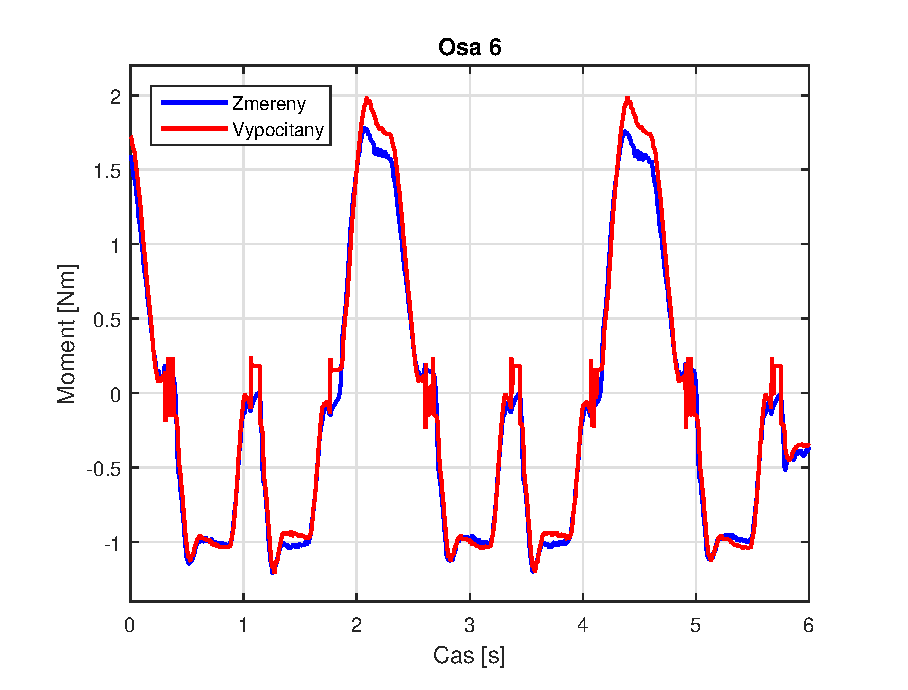
\includegraphics[width=0.6\textwidth]{Osa_6}\label{osa6_prub_a}}
  \hfill
  \subfloat[Okamžitá a průměrná odchylka]{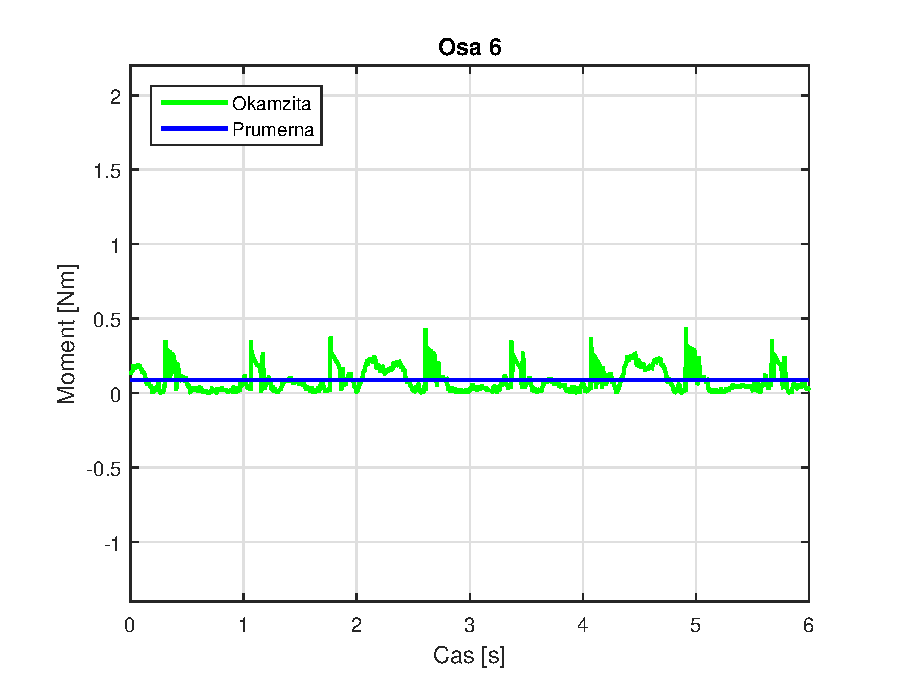
\includegraphics[width=0.5\textwidth]{Osa_6_odch}\label{osa6_prub_b}}
  \caption{Točivé momenty pro osu 6.}
  \label{osa6_prub}
\end{figure}

Stejné průběhy pro osu 5 jsou na obrázku \ref{osa5_prub} a pro osu 4 na obr. \ref{osa4_prub}.

\begin{figure}[!h]
  \centering
  \subfloat[Srovnání naměřených a vypočítaných momentů]{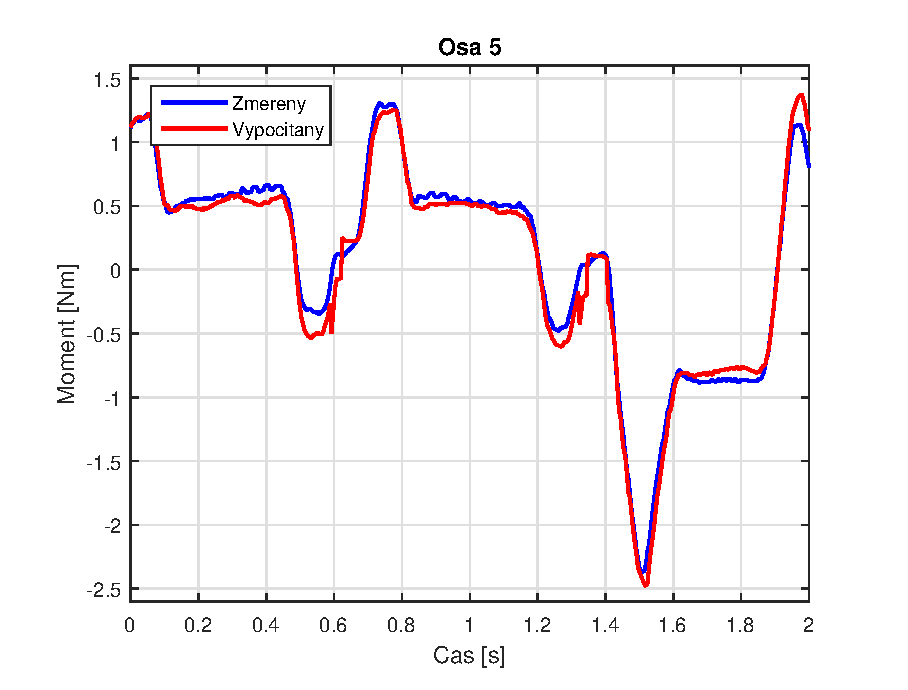
\includegraphics[width=0.5\textwidth]{Osa_5}\label{osa5_prub_a}}
  \hfill
  \subfloat[Okamžitá a průměrná odchylka]{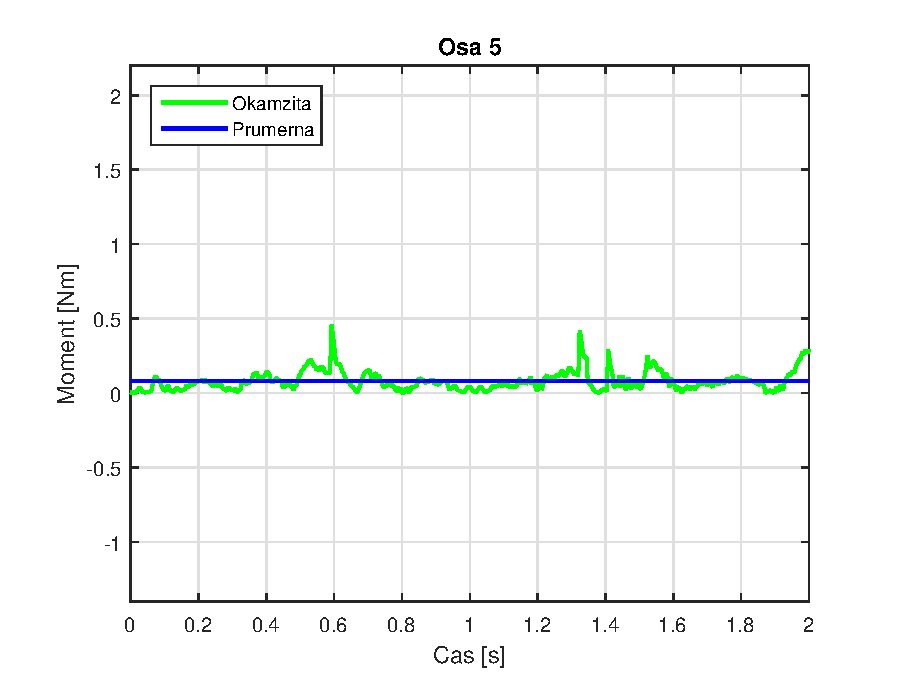
\includegraphics[width=0.5\textwidth]{Osa_5_odch}\label{osa5_prub_b}}
  \caption{Točivé momenty pro osu 5.}
  \label{osa5_prub}
\end{figure}
\newpage

\begin{figure}[!h]
  \centering
  \subfloat[Srovnání naměřených a vypočítaných momentů]{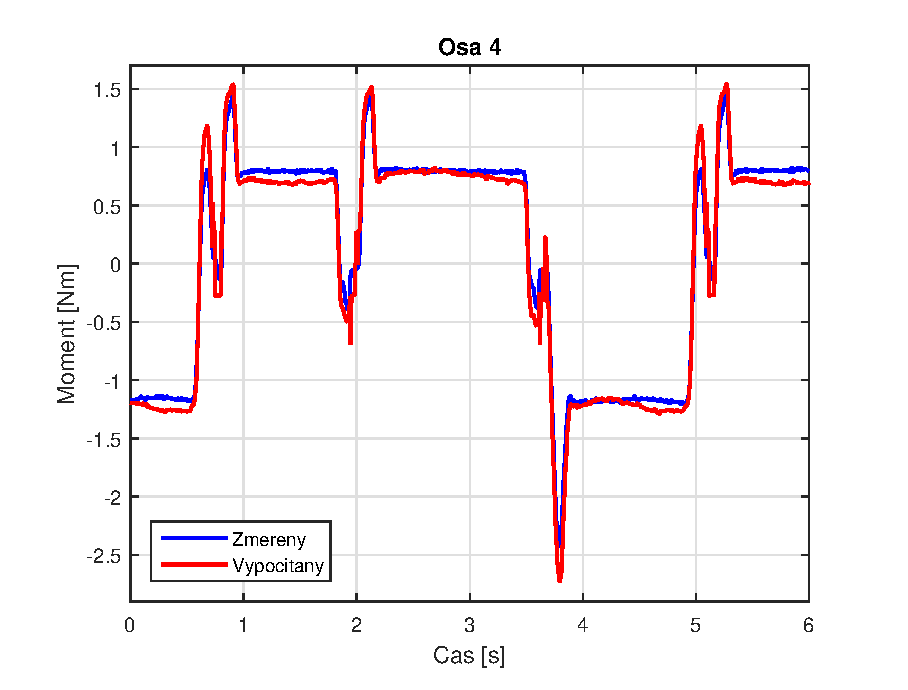
\includegraphics[width=0.5\textwidth]{Osa_4}\label{osa4_prub_a}}
  \hfill
  \subfloat[Okamžitá a průměrná odchylka]{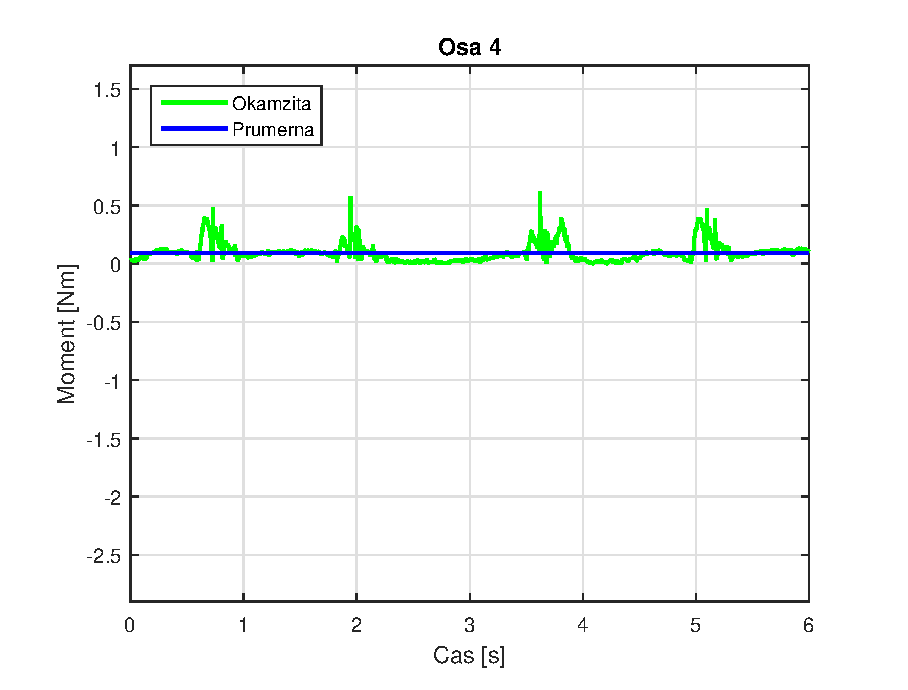
\includegraphics[width=0.5\textwidth]{Osa_4_odch}\label{osa4_prub_b}}
  \caption{Točivé momenty pro osu 4.}
  \label{osa4_prub}
\end{figure}

Z výše uvedených průběhů je patrné, že vypočítané a naměření průběhy si poměrně odpovídají. Ve všech případech se průměrná odchylka pohybuje kolem jedné desetiny Nm a maximální okamžitá odchylka nepřesahuje šest desetin Nm. 

 
\chapter{Srovnání výsledků}

Odvozený a identifikovaný model z kapitoly \ref{identifikovane_parametry_ch}, který dává do vztahu točivé momenty s polohami, úhlovými rychlostmi a úhlovými zrychleními na jednotlivých osách (rovnice \ref{celkova_dyn_rovnice_eq}) je možné použít k výpočtu celkového elektrického výkonu robota (viz sekce \ref{el_vykon_ch}).

Vypočítané momenty sil na jednotlivých osách se pomocí momentových konstant převedly na efektivní hodnoty proudů protékajících vinutími motorů. Nahrazením vinutí motorů obvodem s odporem a indukčností zapojenými v sérii byly z těchto hodnot proudů vypočítány jednotlivé hodnoty efektivního napětí na svorkách motorů. Vynásobením hodnot napětí a proudů byly vypočítány elektrické výkony na jednotlivých osách. Celkový elektrický výkon robota je poté dán součtem všech dílčích výkonů na všech osách.  
\chapter{!!? Vliv odchylek v parametrech !!!!}



Vliv odchylek v hodnotách parametrů na přesnost energetického modelu robotu je analyzován pomocí metody Monte Carlo. Ke každému z parametrů je náhodně přičteno 10 hodnot z rozsahu $p \in [-0.25P_i,0.25P_i]$ se kterými je poté provedena simulace a vypočítaná střední odchylka mezi simulací a změřenými průběhy. Následně je vyhodnoceno, při jakých odchylkách parametrů byl největší rozdíl mezi simulovaným a změřeným průběhem.

\section{Metoda Monte Carlo}

\section{Vyhodnocení}
\chapter{Závěr}

V této práci byly prostudovány způsoby vytvoření modelu šestiosého průmyslového robotu a identifikace jeho dynamických parametrů. Důraz byl kladen na vytvoření metodiky identifikace, kterou by bylo možné použít na široké spektrum typů robotu. 

Tento model by měl sloužit pro modelování spotřeby elektrické energie robotického systému. Z modelu je možné z pohybu při požadovaných robotických operacích predikovat, jaké množství energie tato operace spotřebuje a díky tomu daný proces optimalizovat.

Z hlediska standardizace identifikace dynamických parametrů byly prostudovány a vzájemně porovnány dva postupy, identifikace z 3D modelu robotu a z jeho rovnic. Byly popsány postupy obou způsobů identifikace a analyzovány jejich výhody a nevýhody. 

Dynamické parametry byly také analyzovány z hlediska jejich vlivu na přesnost dynamického modelu robotu. Díky tomu je možné určit, které dynamické parametry mají hrají v přesnosti modelu největší roli a tedy, které parametry je vhodné identifikovat s co nejvyšší přesností.

Pro identifikaci dynamických parametrů z rovnic robotu byl vytvořen skript pro MATLAB, který je schopen vytvořit matematický model, identifikovat jeho parametry, simulovat výsledky a porovnat je s měřením. Skript také umožňuje provádět analýzu vlivu odchylek odhadnutých parametrů na přesnost modelu. 

Data získaná pomocí odvozeného modelu byla porovnána se skutečným reálným měřením. Dále byla provedena analýza důvodů odchylek mezi predikcí a měřením a navrženy způsoby, jak je eliminovat.  

V poslední řadě byla vytvořena aplikace sloužící k exportu dat z databáze dlouhodobého měření energetické spotřeby robotické buňky. Aplikace je schopna provádět zálohu, čištění a export dat z databáze. Byla vytvořena pro zjednodušení a zefektivnění přípravy dat z databáze měření energetické spotřeby robotické buňky používané v závodu společnosti ŠKODA AUTO a.s. v Kvasinách. 

\section{Práce do budoucna}

Za účelem snížení odchylky mezi daty predikovanými pomocí vytvořeného matematického modelu a daty naměřenými způsobem popsaným v této práci je potřeba provést některé úpravy, započítávající vliv frekvenčních měničů a dalších elektrických součástí v rozvaděči robotického systému. 

Jednou z možných úprav je doplnění do modelu robotu rovnic popisujících elektrickou část frekvenčních měničů řídících motory robotu, stabilizátorů napájení a dalších elektrických prvků v elektrickém systému robotu.

Druhou možností je úprava způsobu měření reálné spotřeby robotu tak, aby energie těchto elektrických zařízení nebyla v měření započítána.


%\part{Your Party}

%\blindmathtrue

%\blinddocument

%\begin{table}
%\begin{ctucolortab}
%\begin{tabular}{cc}
%\bfseries Foo & \bfseries Bar \\\Midrule
%foo1 & bar1 \\
%foo2 & bar2
%\end{tabular}
%\end{ctucolortab}
%\caption{Foobar.}
%\label{tab:foobar}
%\end{table}

%\begin{figure}
%\includegraphics[width=0.4\textwidth]{ctu_logo_black}
%\caption{Black logo of the CTU in Pragueueue.}
%\end{figure}

%\begin{figure}[!t]
%\includegraphics[width=0.4\textwidth]{ctu_logo_blue}
%\caption{Blue logo of the CTU in Pragueueue.}
%\end{figure}

%\chapter{Conclusions}

%\section{Test --- this is just a little test of something in the table of contents}

%\subsection{Yes, table of contents}

%\begin{theorem}\begin{enumerate} \item Bla \item Blo \end{enumerate} \end{theorem}


\medskip

%\begin{proof}\begin{enumerate} \item[8] Bla \item Blo \end{enumerate} \end{proof}



\bibliographystyle{abbrvnat}
\renewcommand{\bibname}{Reference}
\bibliography{ctutest}

\appendix
\chapter{Návod k aplikaci MongoDB data exporter}
\label{appendix1}
\section{Kompilace}

Aplikace MongoDB data exporter je napsána v jazyce C. Zdrojový kód aplikace je součástí této práce a je přiložen v souboru ... .

Aplikace je vytvořena jako multiplatformní. Zdrojový kód obsahuje pouze knihovny, které je možné použít na libovolné platformě. Pro vytvoření spouštěče aplikace je nezbytné zdrojové soubory zkompilovat pro použití na dané požadované platformě.

Pro kompilaci pro systém Linux je možné použít vestavěnou sadu kompilátorů GNU Compiler Collection použitím příkazu \texttt{gcc}. Kompilaci pro MS Windows je možné provést například pomocí nástroje Visual Studio příkazem \texttt{cl.exe}. Dynamicky linkované knihovny DLL jsou přiloženy ke zdrojovému kódu.  

\section{Použití}

Aplikace je používána k exportu dat z databáze MongoDB měření elektrického výkonu průmyslových manipulátoru v robotické lince.

Umožňuje uživateli správu záloh databáze (mazání starých záloh, vytvoření nových), export dat ze specifikované databáze a kolekce do určeného souboru a nakonec její čištění.

Aplikaci je možné použít jako vícevláknovou. Uživatel má možnost si zvolit počet vláken použitých pro převod a export dat za účelem zrychlení zpracování velkého množství dat. Každé vlákno poté zpracovává svůj vlastní úsek dat u ukládá jej do samostatného souboru který je označován jako pn (n ... počet vláken). Aplikace podporuje až 16 současně spuštěných vláken. 

Uživatel má dále možnost specifikovat časový úsek, ze kterého chce data exportovat. Prosím vezměte na vědomí, že případě velkého množství dat může určení hranic pro export dat trvat delší dobu. Požadované hranice časového úseku jsou poté přidány do názvu výstupního souboru, aby z názvu souboru bylo možné poznat, jaká data se v něm nachází.

Aplikace se spouští spuštěním souboru \texttt{cl.exe}. Tento soubor je možné spouštět samostatně nebo s následujícími parametry.

Vstupní parametry:

\setlength{\leftskip}{1cm}

\noindent
-h \hspace{0.5cm} - \hspace{0.5cm} Zobrazí nápovědu\newline
-c \hspace{0.5cm} - \hspace{0.5cm} Specifikuje umístění konfiguračnoho soubou

\hspace{0.5cm}Příklad: \hspace{0.5cm} \texttt{run -c C:/files/data/config.conf}

\hspace{0.5cm}přečte konfigurační soubor \texttt{config.conf} umístěný v \texttt{C:/files/data/}

\setlength{\leftskip}{2cm}

V případě, že není uživatelem poskytnuto umístění konfiguračního souboru, je použito výchozí nastavení - \texttt{config.conf} v adresáři souboru \texttt{run}

\setlength{\leftskip}{1cm}
\noindent
-a \hspace{0.5cm} - \hspace{0.5cm} Specifikuje odpovědi na otázky vyskytující se v programu

\setlength{\leftskip}{2cm}
\noindent
Povolené symboly: Y (ano) nebo n (ne)
\newline\noindent
Otázky:

\setlength{\leftskip}{3cm}
\noindent
1. Smazat staré databáze? (Y,n)\newline
2. Vytvořit zálohu vybrané databáze? (Y,n)\newline
3. Exportovat data? (Y,n)\newline
4. Vyčistit vybranou databázi? (Y,n)\newline

\setlength{\leftskip}{2cm}
\noindent
Příklad: \hspace{0.5cm} \texttt{run -a YnYn}

\noindent    
Aplikace spuštěná s těmito parametry smaže staré záložní databáze, nevytvoří nové zálohy, exportuje data a nevyčistí vybranou databázi           

\noindent
Pokud nejsou parametry specifikovány žádné odpovědi, aplikace se spustí normálně a zeptá se na tyto otázky během jejího běhu

\setlength{\leftskip}{0cm}
\noindent
Formát konfiguračního souboru:

\setlength{\leftskip}{1cm}
\noindent
\texttt{URI=mongodb://localhost:27017} - adresa databáze MongoDB \newline
\texttt{DB\_NAME=database} - jméno MongoDB databáze k připojení \newline
\texttt{COLL\_NAME=collection} - jméno kolekce k připojení \newline
\texttt{OUT\_FILE=C:/data\_export.csv} - umístění a název výstupního souboru pro export dat \newline
\texttt{NUM\_THREADS=2} - počet vláken/výstupních souborů pro export dat \newline
\texttt{DATA\_FROM=0} - čas od kterého mají být exportována data \newline
\texttt{DATA\_TO=1701041215} - čas do kterého mají být exportována data \newline

\setlength{\leftskip}{1.5cm}
\noindent
Formát časových hranic: \hspace{0.2cm} RRMMDDhhmm RR-rok, MM-měsíc, DD-den, hh-hodina, mm-minuta                     

\noindent
Pokud nechcete použít časový úsek, zadejte hodnoty 0

\setlength{\leftskip}{1cm}
\noindent 
Aplikace spuštěná s tímto konfiguračním souborem se připojí k databázi MongoDB běžící na místní adrese (localhost) na portu 27010. Dále se pokusí připojit k databázi \texttt{database} a ke kolekci \texttt{collection}. Data budou exportována od začátku až do 4.1.2017 - 12:15. Protože jsou vybrána dvě vlákna, budou vytvořeny 2 výstupní soubory. Data budou exportována do těchto dvou výstupních souborů:

\setlength{\leftskip}{2cm}
\noindent 
\texttt{data\_export\_0-1701041215\_p1.csv} \newline
\texttt{data\_export\_0-1701041215\_p2.csv} \newline
umístěných v \texttt{C:/}



%\printindex

%\appendix

%\ctutemplate{specification.as.chapter}

\end{document}